\documentclass[tikz]{standalone}
\usetikzlibrary{arrows, positioning}
\tikzset{
  treenode/.style = {align=center, inner sep=1pt, text centered,
    font=\sffamily},
  arn_b/.style = {treenode, circle, white, font=\sffamily\bfseries, draw=black,
    fill=black, text width=1.5em},% arbre rouge noir, noeud noir
  arn_r/.style = {treenode, circle, red, draw=red, 
    text width=1.5em, very thick}% arbre rouge noir, noeud rouge
}

\begin{document}
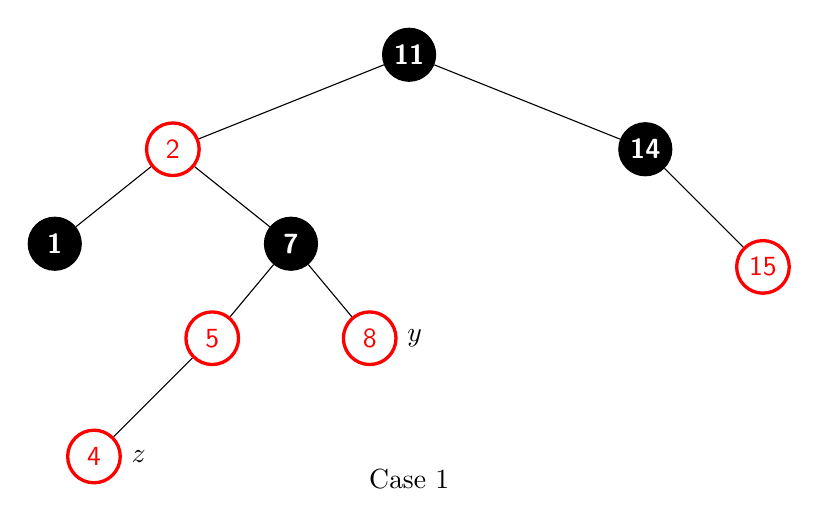
\begin{tikzpicture}[level/.style={sibling distance = 6cm/#1,
  level distance = 1.2cm}] 
\node (root) [arn_b] {11}
    child{ node [arn_r] {2} 
            child{ node [arn_b] {1} 
            }
            child{ node [arn_b] {7}
				child{ node (an5) [arn_r] {5}
                    child{node (an4) [arn_r, below left=of an5] {4}}}
                child{node (an8) [arn_r] {8}}
            }                            
    }
    child{node (an14) [arn_b] {14}
        child{node [arn_r, below right=of an14] {15}}
    }
    ; 
\node [right] at (an4.east) {$z$};
\node [right] at (an8.east) {$y$};
\node [below=of root, yshift=-3.8cm] {Case 1};
\end{tikzpicture}
\end{document}